%%%%%%%%%%%%%%%%%%%%%%%%%%%%%%%%%%%%%%%%%%%%%%%%%%%%%%%%%%%%%%%
%\subsection{Task 2}
%\label{sub:task2}

Task 2 consists in finding all `couples' from a given model, given that two persons are a `couple' if they played together in at least three movies~\cite{imdbcase}. Couples are to be obtained using either from the model obtained in Task 1 or from the IMBd database~\cite{imdbsources}. Once again, we present solutions using e-Motions and Maude.

\subsubsection{e-Motions-based solution}

The solution for this task is implemented with one single rule, \code{createCouple}, shown in Fig.~\ref{fig:createCouple}. \code{Person} objects are shown using square shapes because \code{Person} is an abstract class and it does not have attached image. The \code{createCouple} rule models the creation of a couple by taking two persons and generating a couple with them. The rule has two conditions: a positive condition stating that \textit{``the number of movies in the intersection between the movies of \code{per1} and \code{per2} is greater or equal than 3''}; and a negative condition, the \code{coupleHasNotBeenCreated} NAC, requiring that the couple does not exists yet. 

Although very intuitive and simple, this solution is computationally very expensive. Notice that the number of matchings in the LHS of the rule is combinatorial, leaving all the task to the evaluation of the conditions to accept or discard the couples. 

\begin{figure}[htp]
  \centering
  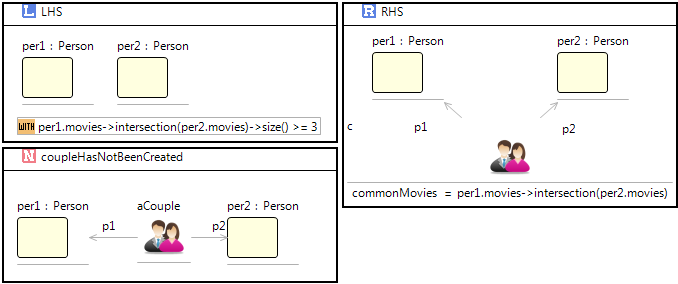
\includegraphics[width=\textwidth]{imgs/ruleCouples}
  \caption{\code{createCouple} rule.}\label{fig:createCouple}
\end{figure}

\begin{table*}[tb]
\renewcommand{\tabcolsep}{6pt}
\renewcommand{\arraystretch}{1.2}
    \centering
	\begin{tabular}[tb]{r|r|r|}
	$N$ & Time (s) & \# Rewrites \\
	\hline
	2 & 0.7 & 524,781 \\
	10 & 46.7 & 19,453,091 \\
	20 & 660.1 & 161,741,321 \\
	\hline \\
	\end{tabular}
	\caption{e-Motions times for Task 2 First Version.}\label{table:emotionstask1}
\end{table*}

We have implemented another solution in which we limit the number of matchings using a very simple algorithm: For each person, we iterate on the rest of persons looking for couples.  
%\begin{enumerate}
%  \item We split \code{Person}s and \code{Movie}s into separate configurations.
%  \item We fix a \code{Person}.
%  \item Given a \code{Person}, we look for all couples.
%  \item Whether the current \code{Person} set has been gone over all the other persons, we set the next person, and the current person is move to the resulting collection.
%\end{enumerate}
With this algorithm, the number of persons to match as candidate couple decreases significantly. To model this solution, we extend the metamodel and its concrete syntax with a so-called \code{Collection} concept. This class has three attributes, namely \code{people}, with the set of persons to be handled, \code{fixedPerson}, to iterate on each person, and \code{peopleDealtWith}, to keep the persons already considered to create a couple with the current `fixed person'. Figures~\ref{fig:initialRule}-\ref{fig:nextPerson} show the rules specifying this solution: 
\begin{itemize}
\item
Rule \code{initialRule} in Figure~\ref{fig:initialRule} initializes the collection object assigning the set of all actors and actresses to its \code{people} attribute (the other attributes get default values). This rule is only fired if there is no collection object in the model. 
\item
Rule \code{fixPerson} in Figure~\ref{fig:fixPerson} takes a person from the \code{people} set and takes it as \code{fixedPerson}. Notice that \code{p} is removed from the \code{people} set.
\item
Rules \code{doingCouples-AreCouple} and \code{doingCouples-AreNotCouple} in Figures~\ref{fig:areCouple} and \ref{fig:areNotCouple} take a person from the set \code{people} and the \code{fixedPerson} and make a couple if the number of movies they share is greater or equal than three. In both cases the person considered is passed to the \code{peopleDealtWith} set. 
\end{itemize}
When all persons has been considered as couple of the current \code{fixedPerson}, the \code{nextPerson} rule, takes the \code{peopleDealtWith} as new \code{people} set. 

\begin{figure}[htp]
  \centering
  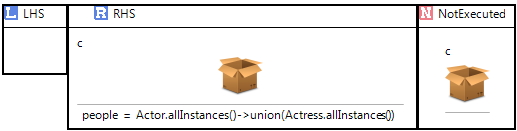
\includegraphics[width=.8\textwidth]{imgs/initialRule}
  \caption{\code{initialRule} rule.}\label{fig:initialRule}
\end{figure}

\begin{figure}[htp]
  \centering
  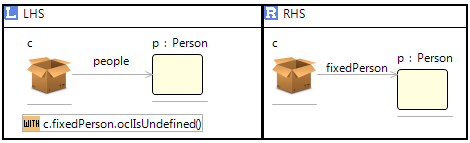
\includegraphics[width=.75\textwidth]{imgs/fixPerson}
  \caption{\code{fixPerson} rule.}\label{fig:fixPerson}
\end{figure}

\begin{figure}[htp]
  \centering
  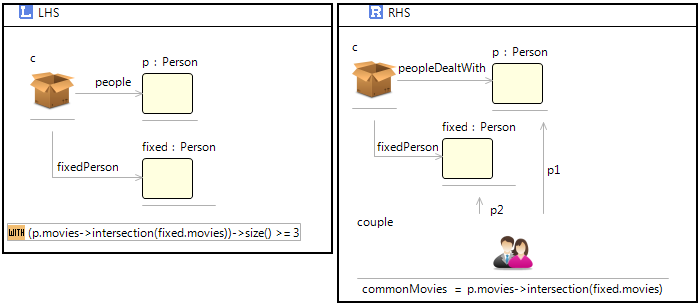
\includegraphics[width=\textwidth]{imgs/areCouple}
  \caption{\code{doingCouples-AreCouple} rule.}\label{fig:areCouple}
\end{figure}

\begin{figure}[htp]
  \centering
  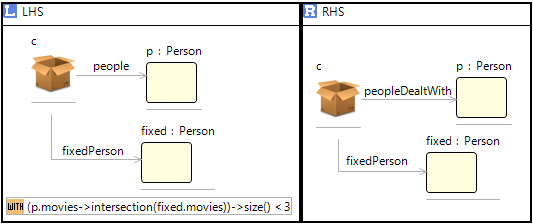
\includegraphics[width=.8\textwidth]{imgs/areNotCouple}
  \caption{\code{doingCouples-AreNotCouple} rule.}\label{fig:areNotCouple}
\end{figure}

\begin{figure}[htp]
  \centering
  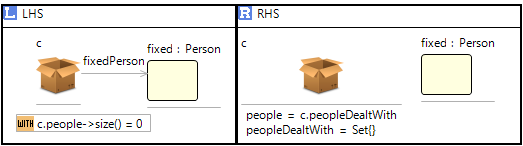
\includegraphics[width=.9\textwidth]{imgs/nextPerson}
  \caption{\code{nextPerson} rule.}\label{fig:nextPerson}
\end{figure}

%!TEX encoding = UTF-8 Unicode\begin{table}
%  \begin{center}
%	\begin{tabular}{r r r}
%	$N$ & Time (s) & \# Rewrites \\
%	\hline
%	2 & 30.105 & 27725365 \\
%	\hline \\
%	\end{tabular}
%	\caption{e-Motions times for Task 2 Second Version.}\label{table:emotionstask22}
%	\end{center}
%\end{table}


\subsubsection{Maude-based solution.}

Again, we specify directly in Maude both solutions. As for Task 1, the solutions match very closely their e-Motions counterparts. 

The Maude solution for the first alternative solution to Task 1 is shown in Listing~\ref{lst:oneRuleCouples}. The rules takes two persons and creates a new couple if they share three movies and such couple has not been previously created. Some numbers for its execution are shown in Table~\ref{table:maudetask21}.
 
\begin{lstlisting}[caption=\code{createCouples} Maude rule., label=lst:oneRuleCouples]
crl [findCouples] :
 { freshOid(N) findCouples
   < O1 : V1:Person | movies : MS1, Atts1 >
   < O2 : V2:Person | movies : MS2, Atts2 > 
   Conf }
=>
 { freshOid(s(N)) findCouples
   < O1 : V1:Person | movies : MS1, Atts1 >
   < O2 : V2:Person | movies : MS2, Atts2 >
   < N : Couple | 
           commonMovies : (intersection((MS1), (MS2))),
           p1 : O1, p2 : O2 > 
   Conf }
if | intersection((MS1), (MS2)) | >= 3
/\ not coupleInConf(C, Conf) .
\end{lstlisting}

\begin{table*}[htb]
\renewcommand{\tabcolsep}{6pt}
\renewcommand{\arraystretch}{1.2}
    \centering
	\begin{tabular}{r r r}
	$N$ & Time (s) & \# Rewrites \\
	\hline
	1 & 0.0 & 8,680 \\
	5 & 0.5 & 1,343,000 \\
	10 & 5.0 & 11,020,000 \\
	20 & 66.3 & 89,276,000 \\
	30 & 314.0 & 302,568,000 \\
	\hline \\
	\end{tabular}
	\caption{Maude times for Task 2 First Version.}\label{table:maudetask21}
\end{table*}

As for e-Motions, the second solutions consists of several rules. In this case, our collection object is model by an operator \code{\{\_\}\{\_\}\{\_\}\{\_\}\{\_\}\{\_\}} representing an object with six attributes as its e-Motions counterpart: the first argument takes the starting argument, the second the people set, the movies set, the dealt people, the fixed person on which to iterate, and the result configuration. We show in Listing~\ref{lst:task2SecondVersion} the code for the \code{doingPairs} rule. In the case of Maude, we only need one rule to consider the positive and negative cases. 

\begin{lstlisting}[caption=\code{doingCouples} Maude rule., label=lst:task2SecondVersion]

rl [doingPairs] :
  < { none }
    { < O1 : V1@Person | movies : MS1, Atts1 >  C1 }
    { C2 }
    { C3 }
    { < O2 : V2@Person | movies : MS2, Atts2 > }
    { freshOid(New) C4 } >
=> 
  < { none }
    { C1 }
    { C2 }
    { < O1 : V1@Person | movies : MS1, Atts1 > C3 }
    { < O2 : V2@Person | movies : MS2, Atts2 > }
    { if | intersection(MS1, MS2) | >= 3 
      then < New : Couple | p1 : O1, p2 : O2, 
              commonMovies : intersection(MS1, MS2), 
              avgRating : 0.0 >
           freshOid(s New)
      else freshOid(New)
      fi 
      C4 } > .
\end{lstlisting}
